\documentclass{article}
\usepackage[margin=1in]{geometry}
\usepackage{amsmath,amsthm,amssymb}
\usepackage{bbm,enumerate,mathtools}
\usepackage{tikz,pgfplots}
\usepackage{chessboard}
\usepackage[hidelinks]{hyperref}
\usepackage{multicol} % Problem 35
\usepackage{xstring} % Difficulty command
\usetikzlibrary{shapes.geometric}

\newenvironment{question}{\begin{trivlist}\item[\textbf{Question.}]}{\end{trivlist}}
\newenvironment{note}{\begin{trivlist}\item[\textbf{Note.}]}{\end{trivlist}}
\newenvironment{references}{\begin{trivlist}\item[\textbf{References.}]}{\end{trivlist}}
\newenvironment{related}{\begin{trivlist}\item[\textbf{Related.}]\end{trivlist}\begin{enumerate}}{\end{enumerate}}

\newcommand\score[1]{
\pgfmathsetmacro\pgfxa{#1+1}
\tikzstyle{scorestars}=[
  star,
  star points=5,
  star point ratio=2.25,
  draw,
  inner sep=3pt,
  anchor=outer point 5
]
  \begin{tikzpicture}[baseline]
    \draw[opacity=0] (0,-0.5) rectangle (0,0.2); % Workaround for whitespace at the bottom.
    \foreach \i in {1,...,4} {
      \pgfmathparse{(\i<=#1?"yellow":"gray")}
      \edef\starcolor{\pgfmathresult}
      \draw (\i*4.5ex,0) node[name=star\i,scorestars,fill=\starcolor]  {};
    }
  \end{tikzpicture}
}

\newcommand{\difficulty}[1]{%
  \IfEqCase{#1}{%
      {1}{
        
\begin{tikzpicture}[scale=0.7, baseline=0.9mm]%
          \definecolor{slopegreen}{rgb}{0.0, 0.5, 0.0}%
          \fill[slopegreen] (0.5,0.5) circle (0.5);%
        \end{tikzpicture}%
      }%
      {2}{
        
\begin{tikzpicture}[scale=0.7, baseline=0.9mm]%
          \definecolor{slopeblue}{rgb}{0.0, 0.44, 1.00}
          \fill[slopeblue] (0,0) rectangle (1,1);%
        \end{tikzpicture}%
      }%
      {3}{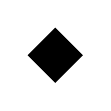
\begin{tikzpicture}[scale=0.7, baseline=0.9mm]\fill (0,0.5)--(0.5, 0)--(1,0.5)--(0.5,1)--cycle; \end{tikzpicture}}%
      {4}{
\begin{tikzpicture}[scale=0.7, baseline=0.9mm]\fill (0.25,0)--(0,0.5)--(0.25,1)--(0.5,0.5)--cycle; \fill (0.75,0)--(0.5,0.5)--(0.75,1)--(1,0.5)--cycle;\end{tikzpicture}}%
      % you can add more cases here as desired
  }[\PackageError{difficulty}{Undefined difficulty level: #1}{}]%
}%
\newcommand{\rating}[2]{\difficulty{#1}\\\score{#2}\\}


\begin{document}
\rating{2}{1}
Suppose that we want to model Plinko/Galton board by supposing that a ball
(1) is equally likely to bounce in either direction off of the first peg, and
(2) will bounce in the same direction that it previously bounced with probability
$p$. For example, when $p = 1$, it will always bounce in the same direction,
when $p=1/2$ it is equally likely to bounce in either direction at any peg, and
when $p=0$, it will alternate left-right-left-right (or vice versa).

\begin{figure}[ht!]
  \scalebox{0.6}{\begin{tikzpicture}
    \foreach \i/\j/\x in {
      0/9/1,
      0/8/1,1/8/1,
      0/7/1,1/7/4,2/7/1,
      0/6/1,1/6/8,2/6/8,3/6/1,
      0/5/1,1/5/12,2/5/28,3/5/12,4/5/1,
      0/4/1,1/4/16,2/4/64,3/4/64,4/4/16,5/4/1,
      0/3/1,1/3/20,2/3/116,3/3/212,4/3/116,5/3/20,6/3/1,
      0/2/1,1/2/24,2/2/184,3/2/520,4/2/520,5/2/184,6/2/24,7/2/1,
      0/1/1,1/1/28,2/1/268,3/1/1052,4/1/1676,5/1/1052,6/1/268,7/1/28,8/1/1
    } {
      \node at (\i + \j/2,\j*0.866) {\small\x};
    }
  \end{tikzpicture}}
  \hfill
  \scalebox{0.6}{\begin{tikzpicture}
    \foreach \i/\j/\x in {
      0/9/1,
      0/8/1,1/8/1,
      0/7/2,1/7/2,2/7/2,
      0/6/4,1/6/5,2/6/5,3/6/4,
      0/5/8,1/5/12,2/5/14,3/5/12,4/5/8,
      0/4/16,1/4/28,2/4/37,3/4/37,4/4/28,5/4/16,
      0/3/32,1/3/64,2/3/94,3/3/106,4/3/94,5/3/64,6/3/32,
      0/2/64,1/2/144,2/2/232,3/2/289,4/2/289,5/2/232,6/2/144,7/2/64,
      0/1/128,1/1/320,2/1/560,3/1/760,4/1/838,5/1/760,6/1/560,7/1/320,8/1/128
    } {
      \node at (\i + \j/2,\j*0.866) {\small\x};
    }
  \end{tikzpicture}}
  \hfill
  \scalebox{0.6}{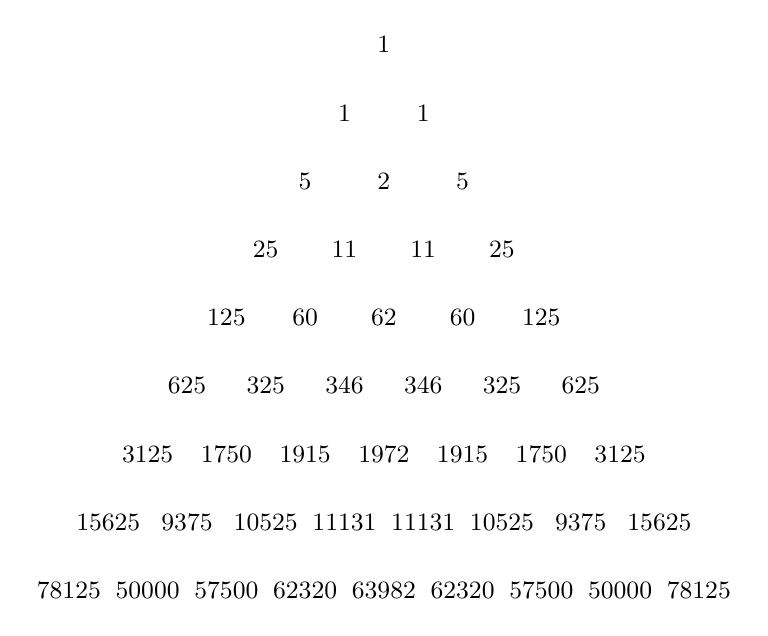
\begin{tikzpicture}
    \foreach \i/\j/\x in {
      0/9/1,
      0/8/1,1/8/1,
      0/7/5,1/7/2,2/7/5,
      0/6/25,1/6/11,2/6/11,3/6/25,
      0/5/125,1/5/60,2/5/62,3/5/60,4/5/125,
      0/4/625,1/4/325,2/4/346,3/4/346,4/4/325,5/4/625,
      0/3/3125,1/3/1750,2/3/1915,3/3/1972,4/3/1915,5/3/1750,6/3/3125,
      0/2/15625,1/2/9375,2/2/10525,3/2/11131,4/2/11131,5/2/10525,6/2/9375,7/2/15625,
      0/1/78125,1/1/50000,2/1/57500,3/1/62320,4/1/63982,5/1/62320,6/1/57500,7/1/50000,8/1/78125
    } {
      \node at (\i + \j/2,\j*0.866) {\small\x};
    }
  \end{tikzpicture}}

  ~

  \noindent
  \includegraphics[width=\textwidth/32*10]{assets/131_problem/p13_10.png}
  \hfill
  \includegraphics[width=\textwidth/32*10]{assets/131_problem/p23_10.png}
  \hfill
  \includegraphics[width=\textwidth/32*10]{assets/131_problem/p56_10.png}
  \caption{
    Illustrations for numerators of $p=1/3$, $p = 2/3$ and $p = 5/6$, followed
    by probably mass functions of the respective tenth rows.
  }
\end{figure}

\begin{question}
  For an arbitrary $p \in [0, 1]$, and a triangle with $n$ rows,
  what is the distribution of balls in bin $k$?
\end{question}

\begin{related}
  \item What is the least/greatest value of $p$ such that at the $(2n)$-th row,
  the middle is equal to the extreme? How about for the $(2n + 1)$-st row?
  \item What if this is done on a different geometry like a cylinder or a
  tetrahedron?
  \item How does this relate to lattice walks? (E.g. see A348595.)
  \item As $n \rightarrow \infty$, does this converge in distribution to a
  normal distribution? If so, what is the variance?
\end{related}

\begin{references}
  \item \href{https://oeis.org/A035002}{A035002: Table of numerators for $p = 2/3$}.
  \item \href{https://oeis.org/A348595}{A348595: Related to table of numerators for $p = 1/3$}.
\end{references}
\end{document}
